\section {Design and Implementation\\}

\subsection{Reactor Model\\}
The PushUp server runs atop of the Twisted framework\cite{Twisted}, an 
event driven framework that implements the ``reactor" style event loop.

The reactor patterns is an event handling pattern for handling concurrent
service requests. It demultiplexes(for example, file descriptor is 
ready for a write operation) these requests to associated event
handlers(implemented as the callback). The event handler then performs
the actual read or write synchronously.

In our project the reactor is implemented as event loops (one Reactor 
can start several event loops) that runs in a single thread. The
Twisted's event loop has well encapsulated the OSes' underlying 
event notification mechanism (kqueue() in Unix and epoll() in Linux).
During execution, the event loop manages the details regarding to
event handler registrations, the activations of event handlers, etc.

The advantage of the reactor patter is the complete separation of the 
application specific code from the reactor implementation. That is to
say, the application components can be easily divided into reusable 
modulars. Also, running the reactor in a single threads significantly
reduce the concurrency controls since no other threads will contend 
the system resource instantaneously.

Figure \ref{fig:mainloop} demonstrates the how the execution switches
between the event loops and user code. Figure \ref{fig:eventloop_flow} 
further illustrates the detailed work flow with sequence diagram.

As we can see from these figures, one of the caveats of in 
event-driven development is that all the event handlers should 
be carefully designed in order to make sure its execution time 
will not take a long time; otherwise the whole system will 
be blocked.

\begin{figure}[htb!]
    \centering%
    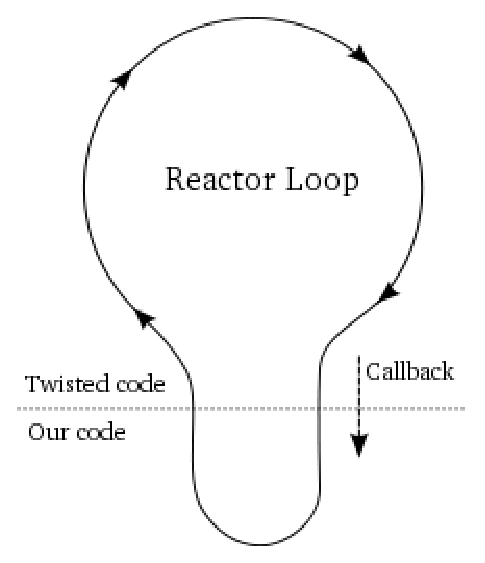
\includegraphics[scale=0.75]{figures/mainloop.eps}
    \caption{Work flow of Twisted Reactor Model}
    \label{fig:mainloop}
\end{figure}
\begin{figure}[htb!]
    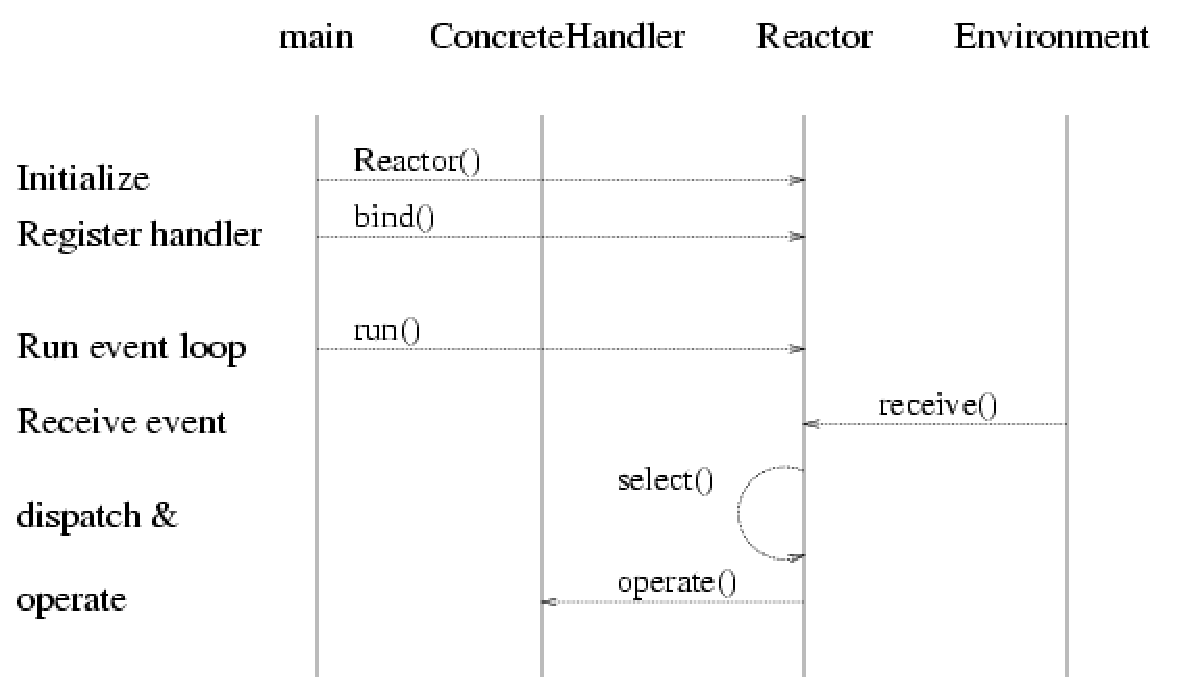
\includegraphics[scale=0.45]{figures/eventloop_flow.eps}
    \caption{The Sequence Diagram of the Event Loop}
    \label{fig:eventloop_flow}
\end{figure}


\subsection{Channels\\}

Metaphor: a channel represents the message stream of a certain topic. For example, the channel can represents the feed of a specific user's tweets in twitter, or the feed of a specific topic.

Responsibilities: manages the subscribers and incoming messages

- Subscriptions: 
    * b-tree, range search
    - Messages: time: 

Periodically purge the timeout users and timeout subscriptions.

\subsection{Message Queue\\}

Manages the channels; manages the subscriptions and xx

Publication: Web server can publish messages to one or more channels (TODO: now the system only supports publishing message to one channel).

    example: in a Q/A community, when a user John posts a new questions with the tags 'c++', 'java'. The questions will be  question will be published to the channel "author: John", "tag:c++" and "tag:java". The newly published message will be assigned with a unique id(TODO: not done yet).

    Subscription: the client sends the subscription to the server with the following information:

    * Interested channels(TODO: only one channel is supported yet)
    * Timeout: the server will keep the connection open for a period for a certain period of time. If nothing happens within that time span, the server will close the connection.
    * <start-time, end-time>: the client can specify the start-time and end-time of the interested messages; everytime the clients receive the latest message they will update the `start-time` in the  next polling request.
    Since same message may be published to several channels, thus it is important to merge the messages from different channels. Since within each channel messages are sorted in <time, id> order, we  can sort messages and remove duplications similar to the merge function in merge sort.

\subsection{Communication between PushUp Servers\\}

Loosely connected to each other, each has exactly the same messages.
Load balancer distributes the requests evenly, for both pub/sub requests.

Information propagation: 
- description:
- Workflow: header

More examples!!

